% Figure: roadmap as presented at TPP 2026 (part 5).
% Build: pdflatex roadmap_tpp.tex  (run inside figures/)
\documentclass[tikz,border=6pt]{standalone}
\usetikzlibrary{positioning,arrows.meta}
\begin{document}
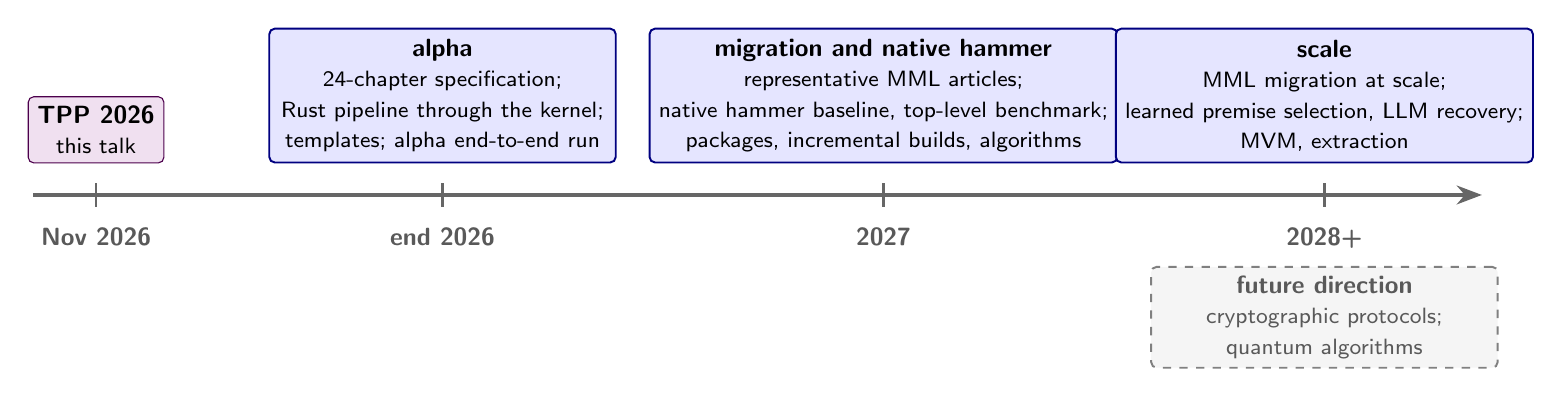
\begin{tikzpicture}[
  font=\sffamily,
  phase/.style={draw, rounded corners=2pt, align=center, minimum width=44mm,
                minimum height=17mm, line width=0.7pt, fill=blue!10,
                draw=blue!50!black, font=\sffamily\small},
  future/.style={phase, dashed, fill=black!4, draw=black!50, text=black!65},
  when/.style={font=\sffamily\small\bfseries, text=black!65},
  axis/.style={-{Stealth[length=3.2mm]}, line width=1.2pt, black!60},
  tick/.style={line width=1pt, black!60},
]
  \draw[axis] (-8mm,0) -- (176mm,0);

  \draw[tick] (0mm,-1.5mm) -- (0mm,1.5mm);
  \node[when, below=3mm of {(0mm,0)}] {Nov 2026};
  \node[draw, rounded corners=2pt, fill=violet!12, draw=violet!60!black,
        align=center, font=\sffamily\small, above=4mm of {(0mm,0)}]
    {\textbf{TPP 2026}\\ \footnotesize this talk};

  \draw[tick] (44mm,-1.5mm) -- (44mm,1.5mm);
  \node[when, below=3mm of {(44mm,0)}] {end 2026};
  \node[phase, above=4mm of {(44mm,0)}]
    {\textbf{alpha}\\ \footnotesize 24-chapter specification;\\
     \footnotesize Rust pipeline through the kernel;\\
     \footnotesize templates; alpha end-to-end run};

  \draw[tick] (100mm,-1.5mm) -- (100mm,1.5mm);
  \node[when, below=3mm of {(100mm,0)}] {2027};
  \node[phase, above=4mm of {(100mm,0)}, minimum width=52mm]
    {\textbf{migration and native hammer}\\ \footnotesize representative MML articles;\\
     \footnotesize native hammer baseline, top-level benchmark;\\
     \footnotesize packages, incremental builds, algorithms};

  \draw[tick] (156mm,-1.5mm) -- (156mm,1.5mm);
  \node[when, below=3mm of {(156mm,0)}] {2028+};
  \node[phase, above=4mm of {(156mm,0)}]
    {\textbf{scale}\\ \footnotesize MML migration at scale;\\
     \footnotesize learned premise selection, LLM recovery;\\
     \footnotesize MVM, extraction};

  \node[future, below=9mm of {(156mm,0)}, minimum height=11mm]
    {\textbf{future direction}\\ \footnotesize cryptographic protocols;\\ \footnotesize quantum algorithms};
\end{tikzpicture}
\end{document}
